\documentclass{beamer}
\usepackage[utf8]{inputenc}

\usetheme{Madrid}
\usecolortheme{default}
\usepackage{amsmath,amssymb,amsfonts,amsthm}
\usepackage{txfonts}
\usepackage{tkz-euclide}
\usepackage{listings}
\usepackage{adjustbox}
\usepackage{array}
\usepackage{tabularx}
\usepackage{gvv}
\usepackage{lmodern}
\usepackage{circuitikz}
\usepackage{tikz}
\usepackage{graphicx}

\setbeamertemplate{page number in head/foot}[totalframenumber]

\usepackage{tcolorbox}
\tcbuselibrary{minted,breakable,xparse,skins}



\definecolor{bg}{gray}{0.95}
\DeclareTCBListing{mintedbox}{O{}m!O{}}{%
  breakable=true,
  listing engine=minted,
  listing only,
  minted language=#2,
  minted style=default,
  minted options={%
    linenos,
    gobble=0,
    breaklines=true,
    breakafter=,,
    fontsize=\small,
    numbersep=8pt,
    #1},
  boxsep=0pt,
  left skip=0pt,
  right skip=0pt,
  left=25pt,
  right=0pt,
  top=3pt,
  bottom=3pt,
  arc=5pt,
  leftrule=0pt,
  rightrule=0pt,
  bottomrule=2pt,
  toprule=2pt,
  colback=bg,
  colframe=orange!70,
  enhanced,
  overlay={%
    \begin{tcbclipinterior}
    \fill[orange!20!white] (frame.south west) rectangle ([xshift=20pt]frame.north west);
    \end{tcbclipinterior}},
  #3,
}
\lstset{
    language=C,
    basicstyle=\ttfamily\small,
    keywordstyle=\color{blue},
    stringstyle=\color{orange},
    commentstyle=\color{green!60!black},
    numbers=left,
    numberstyle=\tiny\color{gray},
    breaklines=true,
    showstringspaces=false,
}
\title 
{MatGeo Assignment 2.6.13}

\author
{AI25BTECH11007}
\begin{document}

\frame{\titlepage}
\begin{frame}{Question}
Given that vectors $\vec{a},\vec{b},\vec{c}$ form a triangle such that
\[
\vec{a}=\vec{b}+\vec{c},
\]
find $p,q,r,s$ given that
\[
\vec{a}=p\hat{i}+q\hat{j}+r\hat{k},\qquad
\vec{b}=s\hat{i}+3\hat{j}+4\hat{k},\qquad
\vec{c}=3\hat{i}+1\hat{j}-2\hat{k},
\]
and the area of the triangle is $5\sqrt{6}$.\\


\end{frame}
\begin{frame}{Solution}
We are given:

\begin{equation}
\vec{a} = \vec{b} + \vec{c}
\end{equation}

\begin{equation}
\vec{a} = p\hat{i} + q\hat{j} + r\hat{k}, \quad
\vec{b} = s\hat{i} + 3\hat{j} + 4\hat{k}, \quad
\vec{c} = 3\hat{i} + 1\hat{j} -2\hat{k}
\end{equation}

and the area of the triangle formed by these vectors is:
\begin{equation}
\text{Area} = 5\sqrt{6}
\end{equation}

\vspace{1em}
\end{frame}
\begin{frame}{Observation:}
For three vectors to form a triangle, they must sum to zero:
\begin{equation}
\vec{a} + \vec{b} + \vec{c} = \vec{0}
\end{equation}

However, we are told:
\begin{equation}
\vec{a} = \vec{b} + \vec{c} \Rightarrow \vec{a} - \vec{b} - \vec{c} = \vec{0}
\end{equation}

This implies:
\begin{equation}
\vec{a} + (-\vec{b}) + (-\vec{c}) = \vec{0}
\end{equation}

So, the triangle is formed by the vectors $\vec{a}, -\vec{b}, -\vec{c}$. For these to form a triangle, they must not lie along the same line (i.e., must not be collinear).

\vspace{1em}
Now, if we assume:
\begin{equation}
\vec{a} = \vec{0}
\Rightarrow \vec{b} + \vec{c} = \vec{0}
\Rightarrow \vec{b} = -\vec{c}
\end{equation}
\end{frame}
\begin{frame}
Given:
\begin{equation}
\vec{c} = \myvec{3 \\ 1 \\ -2} 
\Rightarrow \vec{b} = -\vec{c} = -\myvec{3 \\ 1 \\ -2}
= \myvec{-3 \\ -1 \\ 2}
\end{equation}

Then:
\begin{equation}
\vec{a} = \vec{b} + \vec{c} = \vec{0}
\Rightarrow p = 0,\quad q = 0,\quad r = 0
\end{equation}

We now compute the area of the triangle using:
\begin{equation}
\text{Area} = \frac{1}{2} \left\| \vec{b} \times \vec{c} \right\|
\end{equation}

Compute the cross product:
\begin{equation}
\vec{b} \times \vec{c} = \vec{0} \Rightarrow \text{Area} = 0
\end{equation}

If we assume $\vec{a} = \vec{0}$, then $\vec{b} = -\vec{c}$, and the triangle is degenerate (i.e., the vectors lie on a straight line). Therefore, the area is zero:
\begin{equation}
\boxed{\text{Area} = 0}
\end{equation}
\end{frame}
\begin{frame}{Coclusion}
This contradicts the given area of $5\sqrt{6}$. Therefore, no solution exists such that:
\begin{equation}
\vec{a} = \vec{b} + \vec{c} \quad \text{and} \quad \text{Area} = 5\sqrt{6}
\end{equation}
\end{frame}
\begin{frame}{Plot}
   \begin{figure}[H]
    \centering
    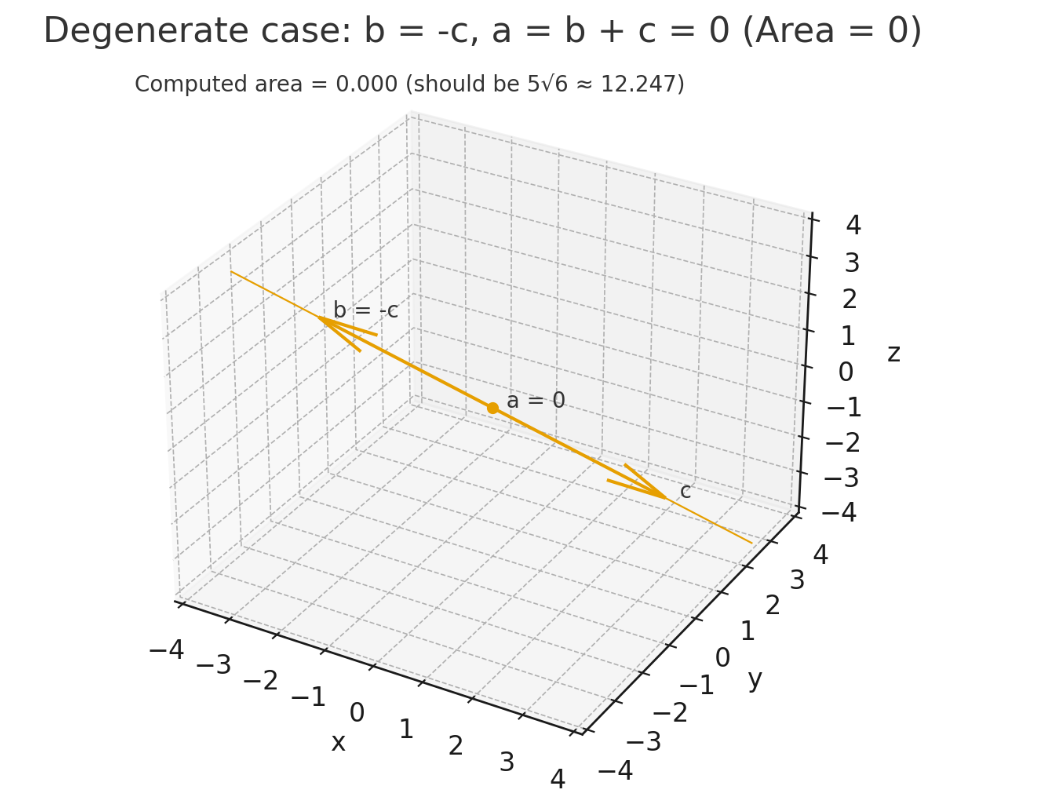
\includegraphics[width=0.75\linewidth]{figs/Screenshot 2025-09-13 191422.png}
    \caption{Image Visual}
    \label{fig:figs/Screenshot 2025-09-13 191422.png}
\end{figure}

\end{frame}
\end{document}